% Tento soubor nahraďte vlastním souborem s obsahem práce.
%=========================================================================
% Autoři: Michal Bidlo, Bohuslav Křena, Jaroslav Dytrych, Petr Veigend a Adam Herout 2019
%-----------------------------------CHAPTER------------------------------------
\chapter{Úvod}
Trend poslední doby byl a stále je neustálé zvětšování obrazovek zařízení i jejich výkonu. Dostali jsme se již do takové fáze, že je tyto zařízení možné využívat obdobně jako klasické počítače a tak je jejich využití pro synchronizaci souborů na snadě.
Vyvíjená aplikace poskytuje systém, který může každý uživatel využít pro svůj účel a svým způsobem. Nejčastěji je \emph{Git} využíván programátory pro verzování souborů vyvíjených programů. Rozšíření \emph{Git LFS} a \emph{Git Annex} pak pro přidání velkých souborů do těchto repozitářů. Jejich využitím se dosáhne efektivity využití prostoru zařízení a současně plného využití systému \emph{Git}. Tyto rozšíření lze ale využívat i samostatně. Například pro ukládání videí nebo i jiných velkých souborů na externí úložiště pro pozdější synchronizaci mezi různými zařízeními různých systémů.

Cílem práce je navrhnout, implementovat a otestovat aplikaci určenou pro operační systém Android. Tato aplikace bude uživateli zprostředkovávat \emph{Git} pro tato zařízení formou přívětivého grafického rozhraní. Dále bude implementovat rozšíření \emph{Git LFS} a \emph{Git Annex} pro práci s velkými soubory. Aplikace je určena zejména vývojářům a jiným pokročilým uživatelům. Je tedy navržena jako maximálně transparentní při zachování prvků jednoduchého ovládání mobilních zařízení.

\newpage
\section{Git}
Git slouží zejména programátorům k verzování jejich práce, popřípadě jejího sdílení s ostatními členy týmu. Nicméně jeho využití je široké a to zejména při využití rozšíření \emph{Git LFS}~\footnote{\label{foot:git-lfs}\url{https://git-lfs.github.com/}} nebo \emph{Git Annex}~\footnoteURL{https://git-annex.branchable.com/}, která se zaměřují na práci s velkými soubory.

\section{Git LFS}
git Large File Storage (LFS) nahrazuje velké soubory v repozitářích ukazateli. Samotné soubory jsou pak uloženy na vzdáleném serveru. Tento systém tedy slouží k efektivnímu uložení velkých souborů v \emph{Git}. Jedná se například o video záznamy, zvukové stopy, datasety a jiné velké binární soubory.

\begin{figure}[h!]
    \begin{minipage}{\textwidth}
    \centering
    \vspace{0.5cm}
    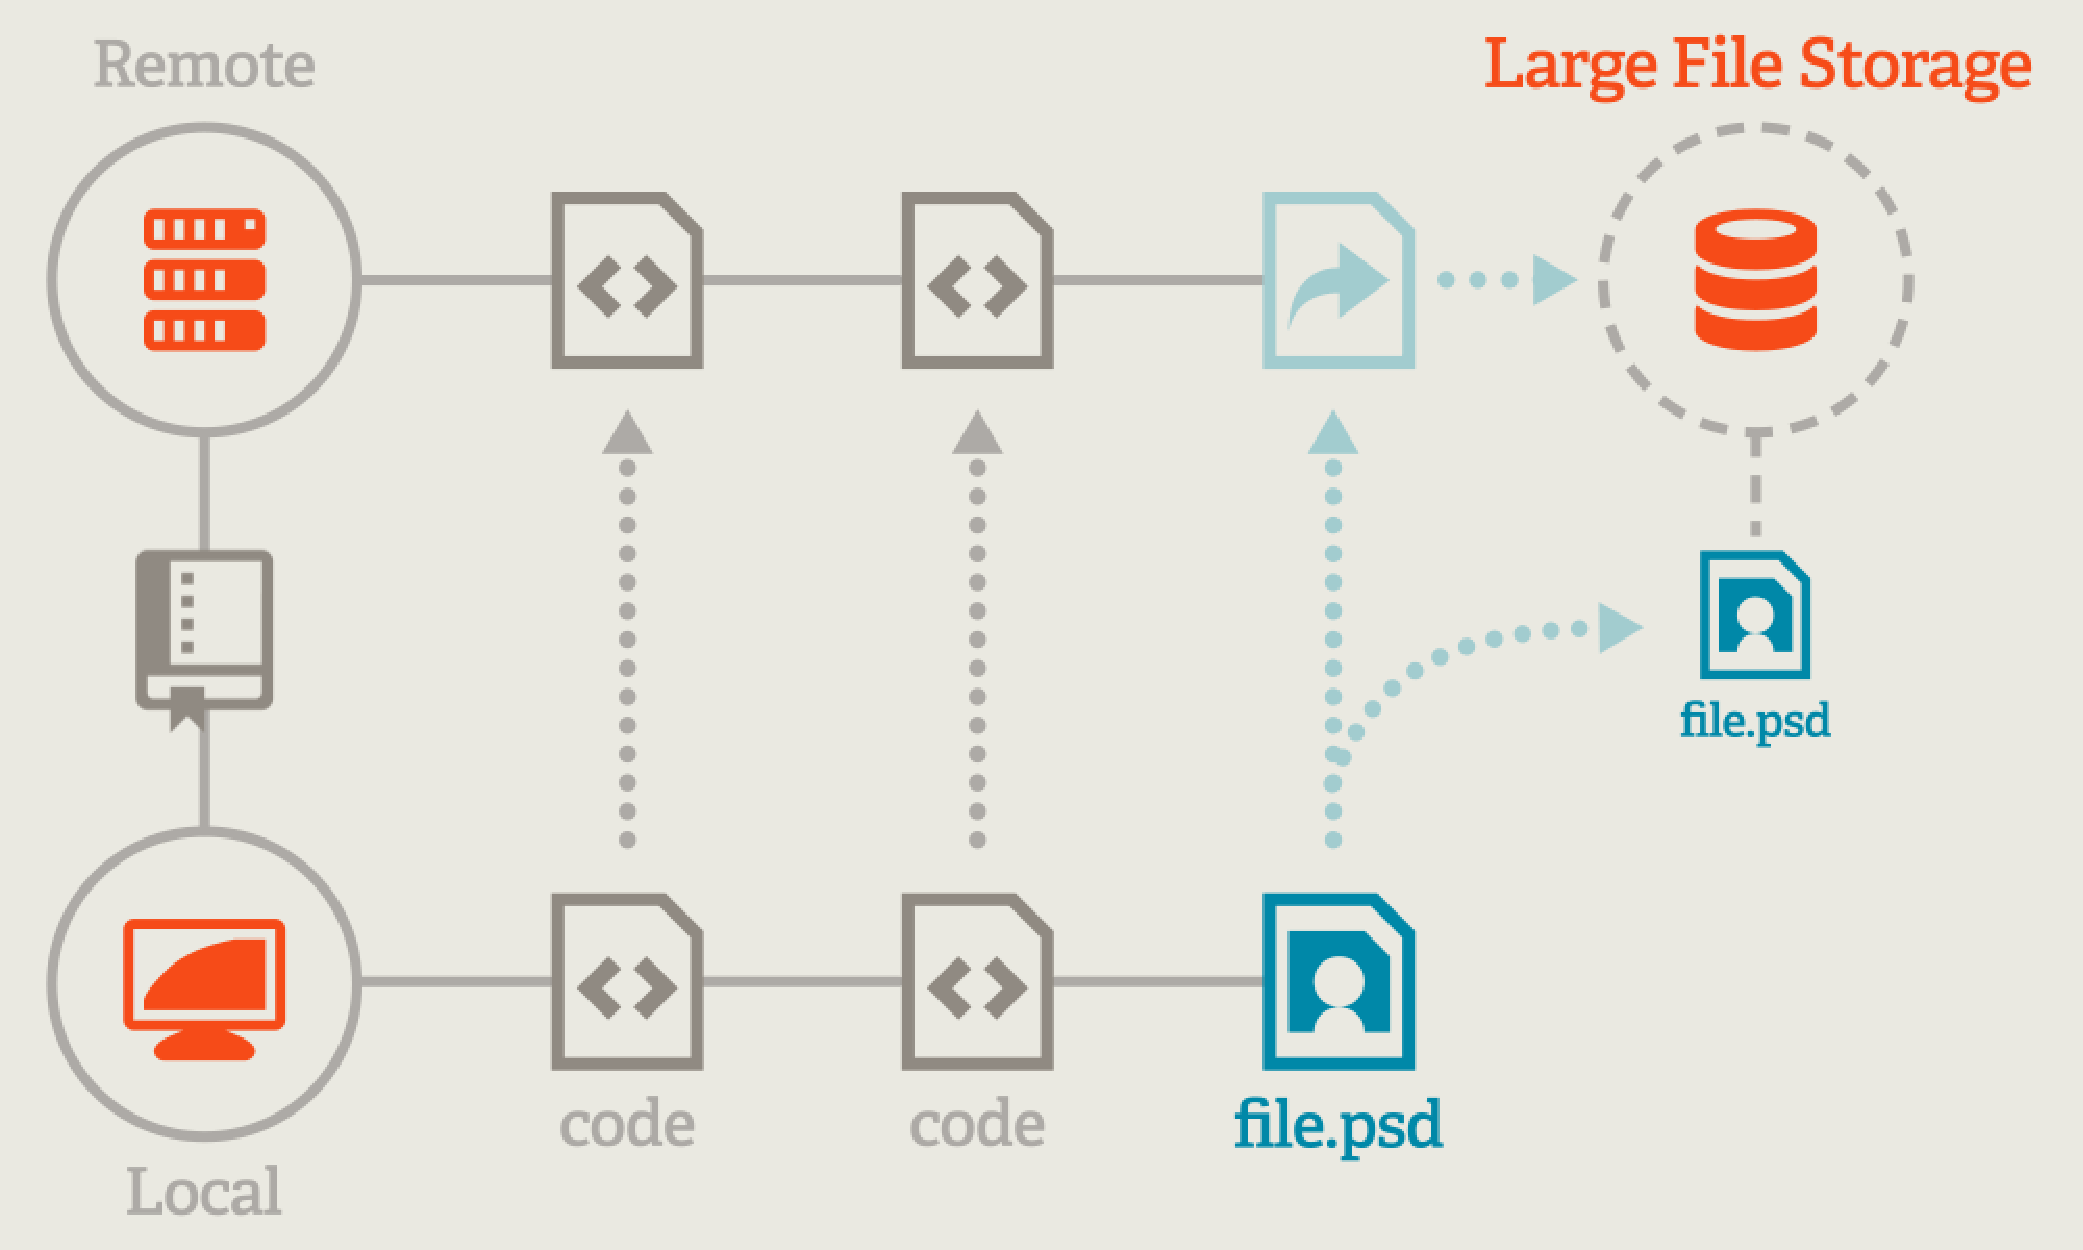
\includegraphics[width=0.75\textwidth,height=0.75\textheight,keepaspectratio]{git-lfs.pdf}
    \caption{Architektura \emph{Git LFS}~\ref{foot:git-lfs}}
    \label{diagram:git-lfs}
    \end{minipage}
\end{figure}

\section{Git Annex}
\emph{Git annex} slouží k indexaci, synchronizaci a sdílení souborů mezi více úložišti nezávisle na komerční službě nebo centrálním serveru~\cite{wiki-git-annex}. V repozitáři je uložen symbolický odkaz na klíč, který je hash daného souboru. Samotný soubor je pak uložen v adresáři \emph{.git/annex/}. Při změně souboru se mění jen jeho hash a aktualizuje symbolický odkaz. Tímto způsobem je zajištěno šetření místa, jelikož samotný soubor je v repozitáři uložen maximálně jednou.

%-----------------------------------CHAPTER------------------------------------
\chapter{Specifikace řešení}
Hlavním cílem aplikace je nabídnout uživatelům řešení pro verzování a synchronizaci velkých souborů jejich \emph{Git} repozitářů na zařízeních systému Android. Priorita tedy bude kladena spíše na funkčnost než perfektní uživatelské rozhraní.

\section{Funkce aplikace}
Aplikace bude mít dvě základní funkce. Jsou jimi správa repozitářů a provádění příkazů \emph{Gitu}. Uživatel bude moci spravovat \emph{Git} repozitáře následujícím způsobem. K přidání nového repozitáře bude mít tři možnosti. Buď může vybrat adresář s daným repozitářem z místních souborů zařízení, inicializovat úplně nový ve zvolené složce nebo klonovat vzdálený. Při otevření repozitáře nad ním může provádět základní příkazy \emph{Gitu} a také některé vybrané funkce již zmíněných rozšíření.

\section{Cílová skupina}
Cílovou skupinou jsou především programátoři nebo i jiní technicky zdatní uživatelé. Ti aplikaci využijí nejčastěji pro prohlížení jejich repozitářů, ale mohou je také jakkoliv měnit a pracovat na nich třeba i z veřejné dopravy. Git annex využijí například při procházení souborů uložených na více fyzických úložištích. Všechny takto sledované soubory budou přehledně zobrazeny v repozitáři a uživatel tak v danou chvíli ani nemusí přemýšlet, kde jsou právě uložené. Jelikož \emph{Git} annex používá jednoduchý formát \emph{Git} repozitáře, je navíc garantováno, že tyto data budou v budoucnu dostupná i bez jeho použití.

\newpage
\section{Průzkum existujících řešení}
Během průzkumu již existující aplikací jsem se zaměřil jak na aplikace operačního systému Android, tak na desktopové operační systémy Linux a Windows.

    \subsection {Android}
    Pro operační systémy Android je trh s řešeními \emph{Gitu} velice omezený. Existují zde několik málo aplikací s podporou pouze pro čtení repozitáře ale i takové, které zvládají i ostatní základní příkazy \emph{Gitu}. Jejich popis a mé postřehy z nich se dočtete na následujících řádkách.

        \subsubsection{MGit~\footnoteURL{https://play.google.com/store/apps/details?id=com.manichord.mgit}}
        Za zmínku z nich stojí MGit. Bohužel neposkytuje podporu pro \emph{Git LFS} ani \emph{Git Annex}. K implementaci příkazů \emph{Gitu} využívá knihovnu \emph{JGit}. Ta sice v aktuální verzi podporuje \emph{Git LFS}, ale v té, kterou aplikace využívá ji ještě nemá. K jejím přednostem patří otevřený kód a velice intuitivní ovládání.
        Úvodní obrazovka aplikace se seznam repozitářů. Po kliknutí na některý se zobrazí obrazovka s jeho detaily. Nalezneme zde správce jeho souborů, log a status repozitáře. Na této obrazovce se také nachází základní ovládací prvek \emph{Gitu} aplikace. Jím je drawer, který se vysunuje z pravé strany obrazovky. V něm jsou obsaženy všechny poskytované příkazy \emph{Gitu}. Tedy jeho užívání není při porozumění obecného užívání \emph{Gitu} nijak náročné. Tato aplikace má integrovaný správce souborů i jejich editování. Ovšem tento editor není dokonalý. Špatně se v něm posouvá kurzor a navíc nemaže konce řádků. Práce s ním je tedy spíše na obtíž. Naštěstí zde autoři přidali i možnost zvolení vlastního editoru z nainstalovaných aplikací.

        \subsubsection{Pocket Git~\footnoteURL{https://play.google.com/store/apps/details?id=com.aor.pocketgit&hl=en}}
        Dále existuje například aplikace \emph{Pocket Git}. Ta je placená a její kód není veřejně přístupný. Využívá integrovaného správce souborů, ale editor již nechává plně na jiných aplikacích. \emph{Pocket Git} má na první pohled přehlednější uživatelské rozhraní. Jednotlivé příkazy \emph{Gitu} rozděluje do různých kategorií a vedle souborů přidává ikonku o jeho stavu. Nicméně \emph{Add} a \emph{Commit} jsou natolik integrované do správce souborů, že jejich správné použití není vůbec intuitivní. Navíc při práci s touto aplikací často narazíte na nejednoznačná chybová hlášení, která neobsahují bližší popis chyby.

        \subsubsection{Termux~\footnoteURL{https://play.google.com/store/apps/details?id=com.termux&hl=en}}
        Pro vývojáře upřednostňující příkazový řádek je možnost instalace aplikace \emph{Termux} a nainstalování \emph{Gitu} do prostředí jeho terminálu. Tam je i možné doinstalovat rozšíření \emph{Git LFS} a \emph{Git Annex}. \emph{Git LFS} lze doinstalovat přímo jako balíček. \emph{Git Annex} je možné stáhnout z jeho oficiálních webových stránek~\footnoteURL{https://git-annex.branchable.com/} a dle návodu~\footnoteURL{https://git-annex.branchable.com/Android/ }uvést do provozu. Obě tato rozšíření lze ovládat z příkazové řádky, přičemž \emph{Git Annex} i přes uživatelské rozhraní. To je implementováno v prohlížeči. Tato webová aplikace je přehledná i pro mobilní zařízení a umožňuje synchronizaci souborů mezi repozitáři různých zařízení.

    \subsection {Desktop}
    Na Linux i Windows existuje mnoho aplikací, které práci s repozitáři zvládají velice dobře. Nicméně prostředí Androidu je od toho desktopového natolik rozdílné, že prostor pro inspiraci je značně omezený.
        \subsubsection{GitKraken~\footnoteURL{https://www.gitkraken.com/}}
        Dobré zkušenosti mám například s aplikací \emph{GitKraken}. Ta zobrazuje repozitář přehledně ve stromové struktuře. V ní lze přímo najetím myši na uzel provádět změny. Příkazy \emph{Gitu} má přehledně zobrazené v horním panelu. Navíc jsou zde dobře řešeny konflikty v souborech. Na jedné straně obrazovky vidíte jednu verzi a na druhé straně druhou. Ve spodní části obrazovky se generuje nová verze. Tu vytváříte postupným procházením obou současných verzí a vybíráním vyhovující varianty. \emph{GitKraken} umí pracovat i s \emph{Git LFS}. K ovládání takto sledovaných souborů používá zvláštní vysouvací nabídku s funkcemi \emph{Git LFS}. Ta se v případě práce s repozitářem podporující toto rozšíření zobrazí vedle základních příkazů. Které soubory takto sleduje lze měnit v nastavení repozitáře nebo při přidávání souborů do stage.

        \subsubsection{Ungit~\footnoteURL{https://github.com/FredrikNoren/ungit}}
        Na první pohled dobrým dojmem působí i aplikace \emph{Ungit}. Ta vás při každé akci naviguje krok po kroku a usnadňuje tak používání \emph{Gitu} pro méně zkušené uživatele. Jedná se o webovou aplikaci založenou na \emph{node.js}. Pro její instalaci je třeba příkazová řádka, pro spuštění pak webový správce. Její hlavní výhoda je tedy nezávislost na platformě. Její ovládání je rychlé, jelikož aplikace zjednodušuje určité procedury \emph{Gitu}. Například sama nabízí \code{Commit} bez nutnosti přidávat soubory do \code{Stage}. Nicméně aplikace tím zapouzdřuje většinu funkcí. Na základní obrazovce kromě stromu změn repozitáře není další ovládací prvek a aplikace se tak v konečném důsledku jeví až příliš uzavřeně.

    \subsection{Zhodnocení průzkumu}
    Z testování aplikací vyplynulo, že nejjednodušší způsob práce s \emph{Git}em je tehdy, když aplikace transparentně zobrazuje příkazy \emph{Gitu} a jejich použití nechá na uživateli. Předejde se tím chybám, jejichž hlášení nejsou vždy dostačující k vyřešení problému. Pokud je funkce dobře zpracována, není třeba vést uživatele krok po kroku. Ovládání se tak urychlí a je stále přehledné.

    Testované mobilní aplikace často využívají vlastní textový editor a správce souborů. V obou případech tyto aplikace integrují velice jednoduché verze a jejich použitelnost je tak značně omezená.

    Dalším bodem jsou chybová hlášení. Těm by měla aplikace pokud možno předcházet. Pokud chybě již není vyhnutí, alespoň by měla mít dobrý popis a nebo i návrh jejího řešení.

    Poslední bod se týká uživatelského rozhraní. Aplikace \emph{MGit} při klonování repozitáře užívá skrývání určitých položek při jejich nadbytečnosti. To je sice užitečný prvek, nicméně při skrytí položky dojde k posunutí těch následujících na její místo a to působí velice rušivě.

%-----------------------------------CHAPTER------------------------------------
\chapter{Vývoj aplikací pro systém Android}
Android je open-source platforma vyvinutá společností \emph{Google}. Její první oficiální verze se dostala na svět 23. Října 2008 a od té doby značně vyspěla. Je založena na systému Linux a většina fyzických zařízení, které ji podporují staví na \emph{arm} architektuře. Android totiž není mířen přímo na konkrétní zařízení tak jako například \emph{iOS} od firmy \emph{Apple}. To přináší mnohé kompromisy, které musí postupovat jak její vývojáři, tak samotní programátoři aplikací. Zařízení se liší svým hardwarem i softwarem. Mají různé velikostí pamětí i displejů.

Při vývoji aplikací pro ni je tedy nutné brát ohled na nejnovější trendy a sledovat procentuální zastoupení kritických parametrů tak, aby výsledná aplikace splňovala zadané požadavky na většině cílových zařízení. To má za následek roztříštěnost aplikací podle mnoha kritérií tak, aby byli plně funkční na co možná největším počtu zařízení. Naštěstí je při vývoji na platformě \emph{Android} k dispozici mnoho nástrojů, se kterými je možné se s těmito problémy vypořádat.

Tato kapitola se zabývá teoretickými základy tohoto systému, které je užitečné mít pro úspěšný vývoj jeho aplikací na paměti. Při získávání přehledu o principu programování Android poslouží zejména oficiální online dokumentace~\footnoteURL{https://developer.android.com/docs} a návody~~\footnoteURL{https://developer.android.com/guide/}. Především z těchto návodů čerpá následující text o základech aplikací. Také je možné najít různou kvalitní tištěnou literaturu. Pro účely programování této aplikace se například osvědčila kniha \emph{Vývoj aplikací pro Android}\cite{android-Lacko}. 

\section{Základy aplikace}
Aplikace pro Android mohou být psány v Kotlinu, Javě, nebo C++. Nástroje Android SDK kompilují kód spolu s ostatními potřebnými daty do APK souboru. Prakticky se jedná o zip archiv, který Android používá pro instalaci aplikací.

Každá aplikace pracuje ve svém vlastním uzavřeném prostoru. Android implementuje princip nejmenších pověření - \emph{principle of least privilege}. Ten zaručuje, že každá aplikace má práva k přístupu jen ke zdrojům, které potřebuje. Další práva lze aplikaci přidat pouze s explicitním souhlasem uživatele.

\section{Android ABI}\label{sec:zaklady_abi}
Různá zařízení mají osazeny různý hardware a tedy i procesory. Různé procesory používají různé instrukční sady. Každá kombinace procesoru a instrukční sady má vlastní aplikační binární rozhraní - \emph{Application Binary Interface (ABI)}. \emph{ABI}~\footnoteURL{https://developer.android.com/ndk/guides/abis} zahrnuje následující informace:
\begin{itemize}
    \item Instrukční sadu.
    \item \emph{Endian} načítání a ukládání paměti. Android je vždy \emph{little-endian}.
    \item Konvenci sdílení dat mezi aplikacemi a systémem.
    \item Formát spustitelných binárních souborů. Android vždy používá \emph{ELF}~\footnoteURL{https://linuxhint.com/understanding_elf_file_format/}.
    \item Formu implementace \emph{C++} kódu \footnoteURL{http://itanium-cxx-abi.github.io/cxx-abi/}.
\end{itemize}

\section{Komponenty aplikace}
Komponenty aplikace jsou základním stavebním blokem každé Android aplikace. Tyto komponenty jsou vstupním bodem aplikace pro uživatele i systém.

    \subsection{Typy komponent}
    Existují čtyři typy komponent:
    \begin{itemize}
        \item \textbf{Activities} - Aktivity
        \item \textbf{Services} - Služby
        \item \textbf{Broadcast receivers} - přijímače vysílání
        \item \textbf{Content providers} - Poskytovatele obsahu
    \end{itemize}

        \subsubsection{Activities}
        Aktivita je vstupní bod uživatele každé aplikace a reprezentuje jednu obrazovku aplikace. Příkladem takové aktivity je seznam přijatých \emph{SMS} zpráv. Po kliknutí na danou zprávu pro její otevření dojde k vyvolání další aktivity, která zobrazuje obsah této zprávy. Jiná aktivita může zajišťovat obrazovku pro odpověď na tuto zprávu, další její přeposlání jinému příjemci. Aktivita zajišťuje následující interakce mezi systémem a aplikací:
        \begin{itemize}
            \item Sledování aktivity uživatele k tomu, aby systém udržoval aktuální proces spuštěný.
            \item Aktivita má přehled o předchozích přerušených aktivitách, ke kterým by se uživatel mohl vrátit.
            \item Při zrušení aktuálního procesu aktivity pomáhá aplikaci k vrácení se do předchozí aktivity.
            \item Poskytuje systému způsob k implementaci přechodů mezi aktivitami
        \end{itemize}

        \subsubsection{Services}
        \emph{Services} nebo také \emph{služby} poskytují způsob pro udržení aplikace běžící na pozadí. Například se jedná o přehrávání hudby, stahování souborů a podobné akce. Tyto dvě akce reprezentují dva různé způsoby využití služeb:
        \begin{itemize}
            \item Přehrávání hudby je akce, kterou uživatel v reálném čase vnímá a systém tak musí její proces prioritně udržovat v chodu.
            \item Stahování souborů nebo jinému zpracování dat na pozadí uživatel nevěnuje veškerou svoji pozornost a proto má systém větší volnost při správě tohoto procesu.
        \end{itemize}
        Pro svoji flexibilitu se \emph{services} staly velice užitečným stavebním blokem různých funkcí systému. Jimi jsou implementovány živá pozadí, upozornění na různé akce, spořiče obrazovky a mnoho dalších.
        
        \subsubsection{Broadcast receivers}
        \emph{Broadcast receiver} je komponenta, která umožňuje systému nebo jiné aplikaci doručit událost cílové aplikaci mimo běžné uživatelské rozhraní. Tyto události může systém aplikaci doručit i pokud zrovna aplikace neběží. Příklad takové události může být upozornění kalendáře na naplánovanou událost. Aplikace kalendáře nemusí běžet, systém přesto tuto událost doručí \emph{broadcast receiveru} aplikace, která toto upozornění zobrazí. \emph{Broadcast receiver} nezobrazuje uživatelské rozhraní, ale může poskytovat upozornění v notifikacích, které uživateli vznik dané události oznámí.

        \subsubsection{Content Providers}
        \emph{Content providers}, v překladu poskytovatelé obsahu, spravují data aplikace. Tyto data mohou být uloženy v souborovém systému, v \emph{SQLite} databázi, na internetu nebo na kterémkoliv jiném trvalém úložišti, ke kterému má aplikace přístup. \emph{Content providers} poskytují rozhraní k přístupu k těmto datům. Tato data jsou identifikována svým \emph{URI} - \emph{Uniform Resource Identifier}. Systém po obdržení daného \emph{URI} rozhodne na základě práv aplikace o přiřazení daného zdroje dat aplikaci. \emph{URI} tedy slouží obdobně jako absolutní cesta v souborovém systému, jen její užití je univerzální.

    \subsection{Aktivace komponent}
    \emph{Activity}, \emph{service} a \emph{broadcast receiver} jsou aktivovány mechanismem zvaným \emph{intent}~\footnoteURL{https://developer.android.com/reference/android/content/Intent}. Ty během chodu aplikace propojují jednotlivé komponenty tak, aby mohly vzájemně spolupracovat. Fungují tedy jako most, přes který si mezi sebou komponenty vyměňují informace.

\newpage
\section{Životní cyklus aktivity}
Protože uživatel má plnou volnost přecházet z a do aplikace, z aktivity do aktivity, je často potřeba pro různé účely detekovat tyto změny stavů. K tomu aktivita poskytuje řadu metod zpětného volání tzv. \emph{callback}. Ty jsou volány v případě, že systém aktivitu vytváří - \textbf{OnCreate()}, přerušuje - \textbf{onPause()}), zastavuje - \textbf{onStop()}, obnovuje - \textbf{onRestart()} nebo ruší - \textbf{onDestroy()}.

\begin{figure}[h!]
    \centering
    \vspace{0.5cm}
    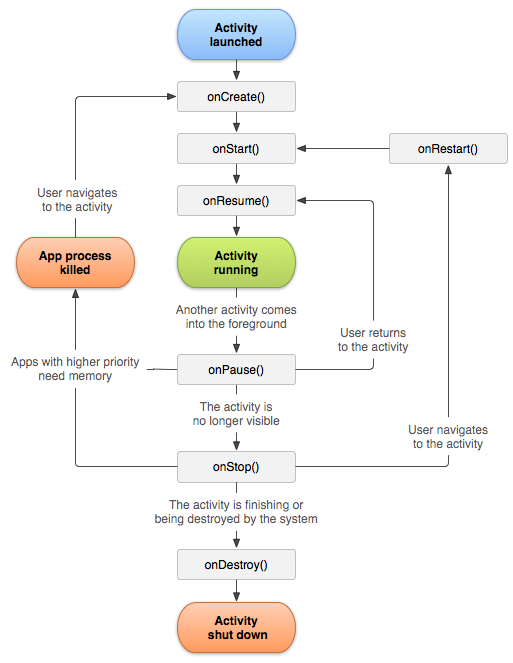
\includegraphics[height=0.7\textheight ,keepaspectratio]{activity_lifecycle_medium.png}
    \caption[Životní cyklus aktivity]{Životní cyklus aktivity~\cite{activity-life-cycle}}
    \label{diagram:activity_lifecycle}
\end{figure}

\newpage
\section{Architektura aplikace}
 Mobilní prostředí aplikací je velice odlišné od toho desktopového, což má vliv na architekturu aplikací. Zejména je to dáno tím, že uživatel často využívá kooperace více aplikací. Například pro sdílení snímků fotoaparátu na sociálních sítích daná aplikace vyvolá \emph{intent} pro spuštění kamery. Ten spustí jinou aplikaci poskytující rozhraní pro pořízení snímku. Tato aplikace po jeho pořízení snímek předá původní aplikaci a ta ho dále zpracovává. Tento způsob práce je pro \emph{Android} typický a aplikace s ním musí umět pracovat.

 Je důležité mít na paměti, že komponenty mohou být spuštěny v různém pořadí a operační systém může jejich běh v jakoukoliv dobu ukončit. Proto by data a stav aplikace neměl být uchováván v rámci těchto komponent.
 
 Tato sekce čerpá informace z oficiálních návodů pro architekturu \emph{Android}~\footnoteURL{https://developer.android.com/jetpack/docs/guide}. Jedná se o doporučenou architekturu pro vývoj mobilních aplikací a aplikace, které se týká tato práce je na ní postavena. Pro implementaci této architektury se využívá knihovny \emph{Android Jetpack}~\footnoteURL{https://developer.android.com/jetpack}.

    \subsection{Základní architektonické principy}
    Existují dva základní architektonické principy. Jejich použití řeší problém kde uchovávat data a stav aplikace tak, aby byly odděleny od uživatelského rozhraní a aplikace byla dobře testovatelná a konzistentní.

        \subsubsection{Oddělení zodpovědnosti}
        Základem této architektury je, aby Aktivita nebo Fragment implementovali pouze logiku týkající se uživatelského rozhraní. To umožní vyhnout se mnoha problémům, které vznikají v rámci životního cyklu aplikace.

        \subsubsection{Uživatelské rozhraní řídí model}
        Dalším důležitým bodem je řídit uživatelské rozhraní z perzistentního modelu. \emph{Model} je komponenta, která má za úkol spravovat data aplikace. Je nezávislá na objektech uživatelského rozhraní a komponent aplikace tak, aby nebyla ovlivněna životním cyklem aplikace.

        \newpage
        \subsection{Doporučená architektura}
        Následující diagram zobrazuje závislosti jednotlivých komponent doporučené architektury. Využitím těchto komponent se dosáhne splnění zmíněných architektonických principů. Tuto architekturu lze také popsat jako \emph{Model, View, ViewModel} - zkráceně \emph{MVVM}.

        \begin{figure}[h!]
            \centering
            \vspace{0.5cm}
            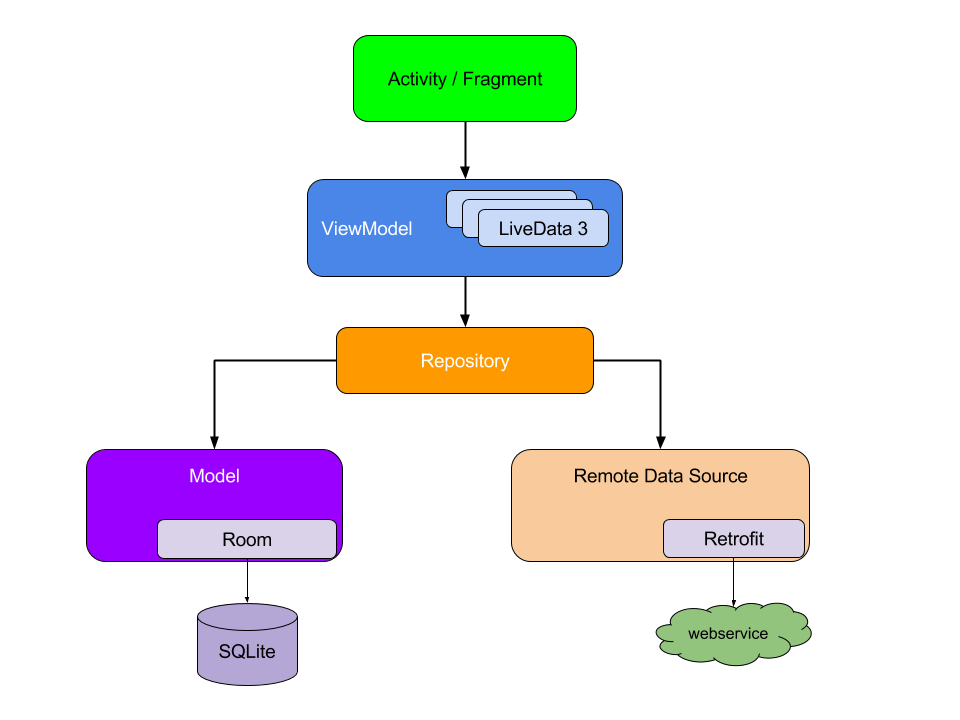
\includegraphics[width=\textwidth, keepaspectratio]{jetpack-architecture.png}
            \caption[Architektura aplikace]{Doporučená architektura~\cite{app-architecture-guide}}
            \label{diagram:jetpack_arch}
        \end{figure}
        
        \begin{enumerate}
            \item Třída \textbf{Activity / Fragment} implementuje logiku uživatelského rozhraní. V terminologii \emph{MVVM} se jedná o \emph{View}.
            \item \textbf{ViewModel}~\footnoteURL{https://developer.android.com/reference/androidx/lifecycle/ViewModel} - třída, umožňující ukládat a spravovat data aplikace nezávisle na jejím životním cyklu.\label{arch:viewmodel}
            \item \textbf{LiveData}~\footnoteURL{https://developer.android.com/reference/android/arch/lifecycle/LiveData} - třída, obsahující data. Je uzpůsobena ke komunikaci mezi aktivitou / fragmentem a \emph{ViewModelem}. 
            \item \textbf{Repository} - třída, poskytující operace nad daty.
            \item \textbf{Model} - třída, definující data databáze.
            \item \textbf{Room}~\footnoteURL{https://developer.android.com/topic/libraries/architecture/room} - knihovna poskytující abstraktní vrstvu nad \emph{SQLite} databází.
        \end{enumerate}

        \subsection{ViewModel}
        Stěžejní částí této architektury je \emph{ViewModel}. Do něj se přesouvá maximum logiky aplikace, data i operace nad nimi. \emph{ViewModel} je inicializován v rámci aktivity nebo fragmentu. Jak již bylo naznačeno v předchozí sekci~\ref{arch:viewmodel}, data uložené v jeho rámci přetrvávají změny stavu spojené s životním cyklem aktivity/fragmentu. Jak dokládá \ref{diagram:viewmodel_lifecycle}, jeho stav zůstává v paměti dokud neskončí jeho aktivita nebo není odpojen jeho fragment.

        \begin{figure}[h!]
            \centering
            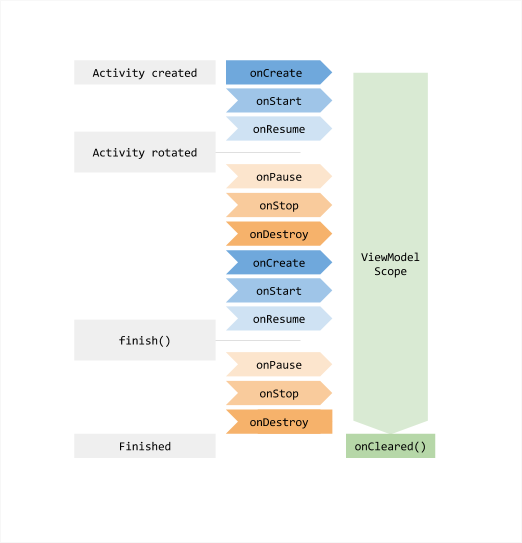
\includegraphics[width=0.8\textwidth, keepaspectratio]{viewmodel-lifecycle.png}
            \caption[Životní cyklus ViewModelu]{Životní cyklus ViewModelu\cite{viewmodel-lifecycle}}
            \label{diagram:viewmodel_lifecycle}
        \end{figure}

        \newpage
        \subsection{Architektonický vzor MVVM}
        Pro správné užití tohoto architektonického vzoru je nutné dodržovat následující závislosti mezi jeho částmi a principy správné komunikace. Pro komunikaci směrem z \emph{View} do \emph{ViewModelu} slouží tzv. \emph{Observer}. Ten sleduje data \emph{LiveData} a při jejich změně vykoná předem definované operace.

        \begin{figure}[h!]
            \centering
            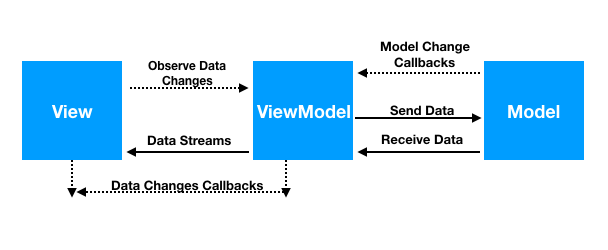
\includegraphics[width=\textwidth, keepaspectratio]{android-mvvm-pattern.png}
            \caption[Vzor MVVM]{Vzor MVVM~\cite{mvvm-pattern}}
            \label{diagram:viewmodel_lifecycle}
        \end{figure}
        
%-----------------------------------CHAPTER------------------------------------
\chapter{Návrh aplikace}
Dle zhodnocení průzkumu i vlastních zkušeností byly na aplikaci stanoveny následující požadavky. Aplikace bude:
\begin{enumerate}
    \item transparentně poskytovat příkazy \emph{Gitu}.
    \item uživatele přehledně informovat o tom co právě dělá, co očekává a jaký je výstup.
    \item využívat externí správce souborů.
    \item mít co nejmenší počet za sebou následujících aktivit a tedy i přechodů mezi nimi.
\end{enumerate}

\section{Funkce aplikace}
Git je velice komplexní systém a proto hrozí, že jeho plná implementace by na zařízeních android byla velice nepřehledná. Vybrány byly tedy nejdůležitější funkce, které jsou nutné pro prohlížení a úpravu repozitářů. 

    \subsection{Správa repozitářů}
    Po spuštění aplikace uživatele uvítá obrazovka se seznamem sledovaných repozitářů. Repozitář je možné do něj přidat několika způsoby. Prvním je přidání již existujícího repozitáře specifikováním jeho cesty v úložišti zařízení. Druhým je klonování nebo inicializace repozitáře z prostředí aplikace. Tento seznam repozitářů je synchronizován s úložištěm zařízení. Příkazy \emph{Gitu} bude moci uživatel provádět po otevření daného repozitáře.

    \newpage
    \subsection{Příkazy Gitu}
    Jelikož žádné aplikace pro Android kromě \emph{Termux} neimplementují rozšíření \emph{Git Annex} a nenalezl jsem knihovnu, která by toto dokázala, bylo rozhodnuto pro příkazy \emph{Gitu} využít zkompilované binární soubory. Mezi tyto funkce patří i funkce rozšíření. Všechny tyto příkazy budou dostupné při otevření repozitáře v bočním výsuvném panelu aplikace. Pro transparentní zobrazení stavu repozitáře budou tyto funkce zobrazovat i svůj klasický textový výstup.

        \subsubsection{Git}
        Pro umožnění základního užití nástroje \emph{Git} budou uživateli dostupné následující příkazy:
        \begin{itemize}
            \item \textbf{\code{add}} - přidání souborů do \emph{stage}
            \item \textbf{\code{commit}} - vytvoření nového \emph{commitu} - potvrzení změn a vytvoření nového uzlu \emph{Gitu}
            \item \textbf{\code{push}} - nahrání obsahu nových \emph{commitů} na vzdálený server
            \item \textbf{\code{pull}} - stažení obsahu nových \emph{commitů} ze vzdáleného serveru
            \item \textbf{\code{status}} - výpis stavu souborů repozitáře
            \item \textbf{\code{log}} - detailní výpis \emph{commitů} repozitáře
            \item \textbf{\code{reset --hard}} - obnova změněných souborů, které ještě nejsou součástí aktuálního uzlu
            \item \textbf{\code{remote add origin}} - přidání \emph{URL} nového vzdáleného serveru
            \item \textbf{\code{remote set-url origin}} - editace \emph{URL} aktuálního vzdáleného serveru
            \item \textbf{\code{branch}} - výpis větví
            \item \textbf{\code{checkout <branch>}} - přepnutí z aktuální větve na větev \code{<branch>}
            \item \textbf{\code{checkout --track <branch>}} - stažení obsahu vzdálené větve a přepnutí z aktuální větve na tuto novou větvi
        \end{itemize}

        \subsubsection{Git LFS}
        Pro rozšíření \emph{Git LFS} pak budou dostupné tyto příkazy:
        \begin{itemize}
            \item \textbf{\code{track <pattern>}} - přidání souborů, které odpovídají regulárnímu výrazu \emph{pattern} sledovaných souborů
            \item \textbf{\code{untrack <pattern>}} - ukončení sledování souborů daných výrazem \emph{pattern}
            \item \textbf{\code{track}} - výpis sledovaných výrazů
            \item \textbf{\code{ls-files}} - výpis sledovaných souborů 
            \item \textbf{\code{status}} - výpis stavi repozitáře s \emph{Git LFS}
            \item \textbf{\code{env}} - výpis prostředí \emph{Git LFS}, pro hledání řešení chyb repozitáře
        \end{itemize}
    
\section{Použité technologie a nástroje}
Před samotným programováním aplikace bylo třeba udělat průzkum nástrojů, které se při vývoji na zařízení Android používají. Tyto nástroje byly vybrány s důrazem na efektivitu vývoje i náročnost jejich použití. Nejdůležitějším z nich je \emph{Android Studio}~\footnoteURL{https://developer.android.com/studio}. Pro verzování byl použit nástroj \emph{Git}, prostřednictvím aplikace \emph{GitKraken}~\footnoteURL{https://www.gitkraken.com/}. Kód aplikace byl synchronizován se vzdáleným repozitářem na serveru \emph{GitHub}~\footnoteURL{https://github.com/}. Pro dynamické generování instalačních souborů aplikace byl repozitář navíc synchronizován s \emph{GitLab CI/CD}~\footnoteURL{https://docs.gitlab.com/ee/ci/}. Pro vytváření binárních souborů \emph{Gitu} a \emph{Git} LFS byl použit \emph{Docker}~\footnoteURL{https://www.docker.com/}. Obraz pro jejich kompilace poskytuje aplikace \emph{Termux packages}~\footnoteURL{https://github.com/termux/termux-packages}.

\section{Architektura aplikace}
Aplikace je psána v jazyce \emph{Java}. Dále využívá návrhového vzoru \emph{Model–view–viewmodel} (dále jen~\emph{MVVM}). K implementaci této architektury využívá knihovny \emph{Android Jetpack}~\footnoteURL{https://developer.android.com/jetpack}.

    \subsection{Kotlin vs. Java}
    Od 7. května 2019 se \emph{Kotlin} stal preferovaným jazykem vývoje pro Android. Proto jsem od začátku plánoval programovat aplikaci právě v něm. Nicméně během programování aplikace jsem zjistil, že naprostá většina zdrojů na internetu pro řešení problémů pro tuto platformu je psána v Javě. Android studio sice umožňuje zkonvertovat kód do Kotlinu, nicméně ani to není to vždy dokonalé. Užití Kotlinu má tu výhodu, že dovoluje programátorovi vynechat určité části kódu, které jsou nutné pro běh aplikace, ale přímo neřeší daný problém. V angličtině se pro ně vžil výraz \emph{boilerplate code}. Ovšem tento kód je přesto třeba vygenerovat, ale o to se již stará Kotlin. To je také jeden z důvodů, proč Kotlin trvá déle zkompilovat. Pokročilým Android vývojářům jistě přijde rychlejí práce vhod, ale jako začínají programátor na této platformě více ocením transparentnost Javy.

    \newpage
    \subsection{Databáze}
    Databáze je využívána pro získání přehledu o repozitářích \emph{Gitu}, které chce uživatel aplikací sledovat. Každý takový repozitář je reprezentován entitou databáze \code{Repo}. Tato tabulka obsahuje absolutní cestu ke složce repozitáře, URL vzdáleného repozitáře, uživatelské jméno a heslo pro přístup k němu. Všechny tyto položky je třeba při provádění příkazů \emph{Gitu} aktualizovat tak, aby stav entity v okamžitém časem odpovídal stavu repozitáře.

    \begin{figure}[h!]
        \centering
        \vspace{0.5cm}
        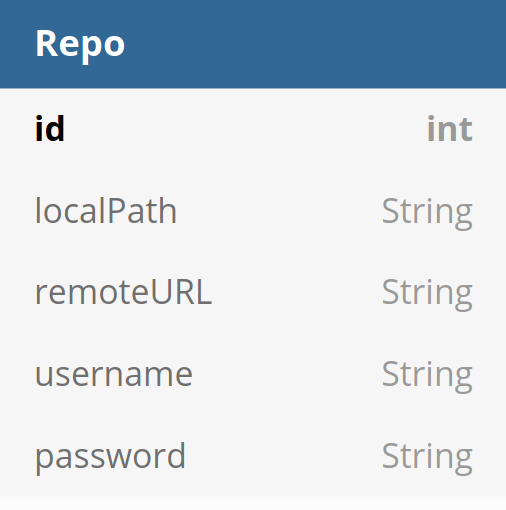
\includegraphics[width=0.3\textwidth,height=0.3\textheight,keepaspectratio]{Repo.png}
        \caption{Entita repozitáře}
        \label{RepoTable}
    \end{figure}

    \subsection{Návrhový vzor}
    \emph{Model–view–viewmodel} je v době psaní této práce doporučovaným návrhovým vzorem Android aplikací. K volbě tohoto návrhového vzoru dopomohlo také využití knihovny \emph{Room}. Tato knihovna totiž spoléhá na využití \emph{MVVM} vzoru alespoň pro účely funkčnosti databáze. Je tomu tak proto, že data, která závisí na databázi se ukládají do proměnné datového typu \emph{LiveData}. Hodnotu této proměnné lze sledovat a na jejím základě řídit běh aplikace. Aby byla hodnota této proměnné perzistentní při běhu aplikace, uchovává se její hodnota ve \emph{viewmodelu}. Hlavní takovou proměnnou je v této aplikaci seznam všech \emph{Git} repozitářů, \code{mAllRepos}, který se nachází ve třídě \code{RepoRepository}.
    
    \subsection{Obrazovky Aplikace}
    Aplikace bude rozdělena podle obrazovek do aktivit. Tyto aktivity dále mohou obsahovat různé fragmenty. Ke každé aktivitě, která poskytuje určitou obrazovku je připojen její ViewModel. Ten jí poskytuje data a funkcionalitu. Vzhled obrazovky je dán jejím \emph{layoutem}.

    \newpage
    \subsection{Dělení aplikace do balíčků}
    Podle zaměření tříd je aplikace dělena do třech základních balíčků. Jsou jimi \code{java}, \code{cpp}, a \code{res}. V balíčku \code{java} je specifikováno chování aplikace. Hlavním obsahem balíčku \code{cpp} jsou archivy s binárními soubory \emph{Gitu} a program \code{bootstrap.c} pro jejich instalaci. Posledním balíčkem je \code{res}. Ten obsahuje všechny \emph{layouty}, ikony a další grafické i textové prvky, které aplikace používá pro grafické rozhraní.

    Následující popis funkčnosti a závislostí balíčků se bude týkat balíčku \code{java}. Záměrně byl z diagramu vynechán balíček \code{utilities}. Jeho třídy lze použít kdekoliv v aplikaci a pro budoucí vývoj aplikace jeho zahrnutí nemá opodstatnění.

    \begin{figure}[h]
        \centering
        \vspace{0.5cm}
        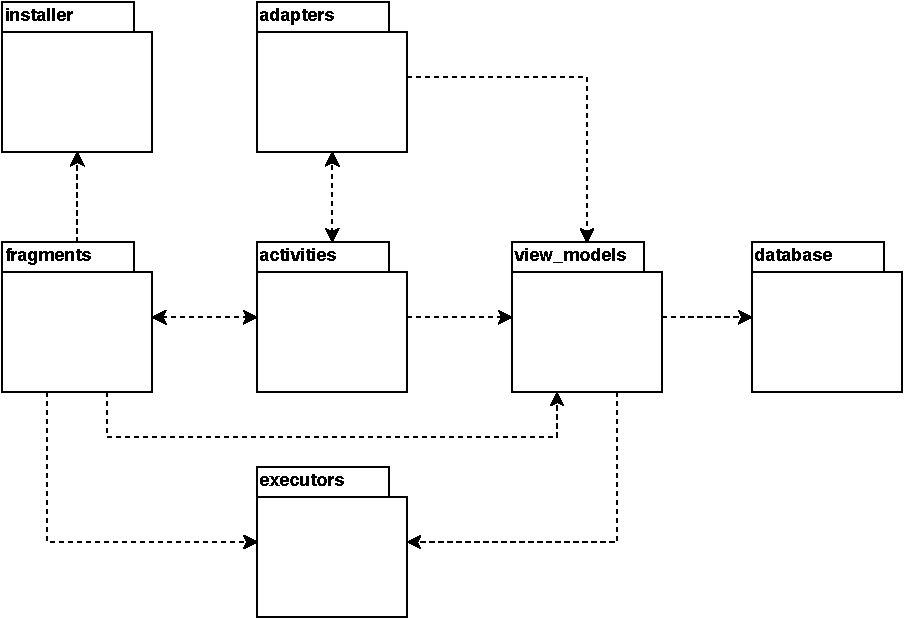
\includegraphics[]{drawio/package_diagram.pdf}
        \caption[Diagram závislostí balíčků]{Diagram závislostí balíčků}
        \label{diagram:packages}
    \end{figure}

    \newpage
    \subsubsection{activities}
    Nejdůležitější součást balíčku \code{Java} je balíček \code{activities}. Ten aplikaci dělí na obrazovky a o každou z nich se stará jedna třída. Tedy v případě, že aplikace potřebuje určitou obrazovku, je zavolána příslušná aktivita s jejím chováním. Všechny aktivity aplikace rozšiřují základní aktivitu \code{BasicAbstractActivity}. Ta implementuje společné prvky rozhraní aktivit. Například získávání oprávnění, zobrazení různých oznámení a dialogů.

    \subsubsection{adapters}
    Tento balíček obsahuje třídy, které slouží k zobrazení položek stejného typu. Tato aplikace je využívá k zobrazení seznamu repozitářů základní obrazovky a příkazů \emph{Gitu} v bočním výsuvném panelu. Adaptér \code{RepoTasksAdapter.java} pro zobrazení tohoto výsuvného panelu byl převzat z implementace aplikace \emph{MGit} třídy \code{RepoOperationsAdapter.java}~\footnoteURL{https://github.com/maks/MGit/blob/master/app/src/main/java/me/sheimi/sgit/adapters/RepoOperationsAdapter.java} a následně upraven pro potřeby aplikace.

    \subsubsection{database}
    Tento balíček obsahuje balíček \code{model}, ve kterém se nachází třída Repo. Ta implementuje tabulku databáze uchovávající všechny potřebné informace o repozitáři. Instance databáze se uchovává ve třídě \code{RepoDatabase}. K přístupu k ní se využívá třída \code{RepoDao}. Tato třída obsahuje metody volající \emph{SQLite} dotazy databáze. Aplikaci je databáze zprostředkována třídou \code{RepoRepository}, která odpovídá \code{Repository} modelu~\emph{MVVM}. Databáze se ukládá do bezpečného vnitřního prostoru balíčku aplikace.

    \subsubsection{fragments}
    Fragmenty, třídy které dynamicky rozšiřují nebo mění obsah aktivity. Aplikace používá fragmenty například k instalaci a nastavení. Každá aktivita může obsahovat několik fragmentů, které samostatně řeší určitou část aktivity.

    \subsubsection{install}
    O instalaci binárních souborů se stará třída \code{InstallTask} v balíčku \code{install}. Ta při prvním spuštění aplikace zkopíruje potřebné soubory ze složky \code{cpp} do interní paměti zařízení.

    \subsubsection{executors}
    Základní příkazy \emph{Gitu} i jeho rozšíření jsou implementovány v balíčku \code{executors}. Tyto jednotlivé příkazy implementují metody třídy \code{GitExec}. Tyto metody volají metodu \code{run} třídy \code{BinaryExecutor} využívající \code{ProcessBuilder}. Ta spustí binární soubor, který vykoná daný příkaz na zařízení.

    \subsubsection{utilities}
    Jedná se o třídy, metody a proměnné, které je možné použít kdekoliv v aplikaci.

    \newpage
    \subsubsection{view\_models}
    Třídy obsahující perzistentní data a implementující logiku nad nimi. Tento balíček odpovídá části \emph{ViewModel}~\emph{MVVM} a poskytuje aplikaci metody zajišťující její funkčnost. Komunikace mezi třídami ViewModelů a aktivitami je zajištěna pomocí \emph{databindingu}, \emph{observerů} a veřejných metod, které tyto třídy poskytují.

    \begin{figure}[h]
        \centering
        \vspace{0.5cm}
        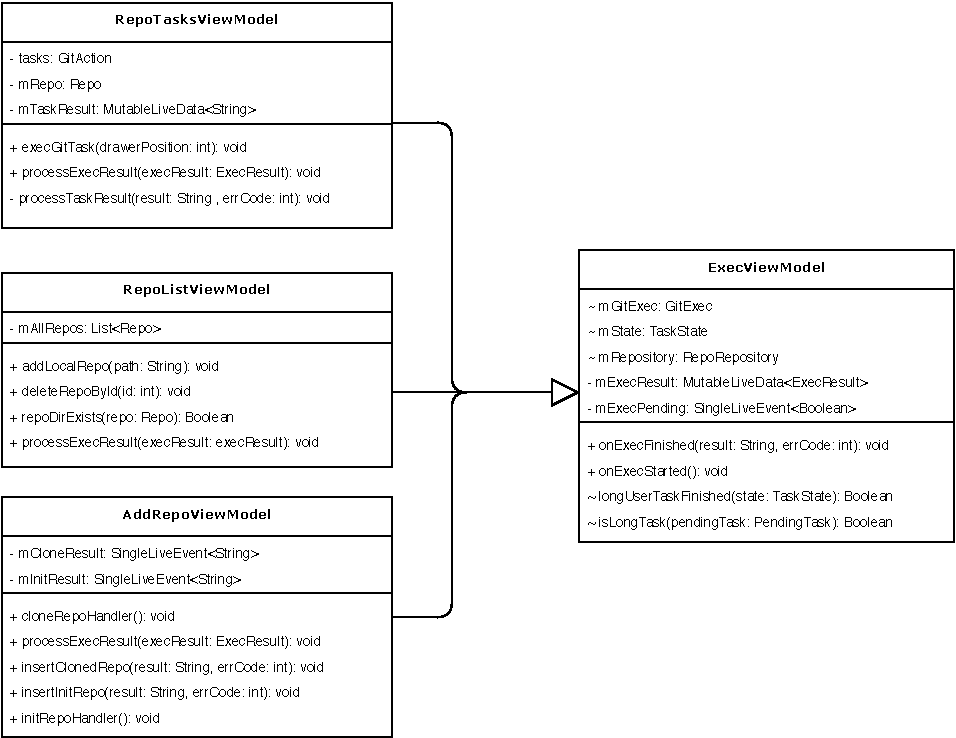
\includegraphics[]{drawio/viewmodels_class_diagram.pdf}
        \caption[Diagram závislostí tříd view modelů]{Diagram závislostí tříd view modelů. Pro přehlednost byl zahrnut jen výběr stěžejních atributů a metod těchto tříd.}
        \label{diagram:view_models}
    \end{figure}

\newpage
\section{Grafické uživatelské rozhraní}
Významnou součástí řešení mobilní aplikace je i její uživatelské rozhraní. To bylo navrženo s důrazem na užití \emph{Material Designu}~\footnoteURL{https://material.io/}. Uživatelé Android jsou na něj zvyklí z většiny populárních aplikací a orientace v něm je tedy pro ně bezproblémová.

Grafické rozhraní se nejvíce inspiruje aplikací \emph{MGit} a přidává prvky vzniklé z požadavků na aplikaci. Především se jedná o přidání příkazů rozšíření a změnu rozhraní pro práci s repozitářem. Uživateli bude po volání příkazů \emph{Gitu} sdělen přesný textový výstup, který mu poslouží pro další práci s \emph{Gitem}. 

Nejprve byly na papír navrženy velice jednoduché wireframy pro ujasnění obsahu nejdůležitějších obrazovek. Ty byly postupně testovány a přepracovávány tak, aby poskytly přívětivé ovládaní aplikace. Poté byly tyto výsledné obrazovky naprogramovány přímo v Android studiu a užity pro první prototypy aplikace. Ukázka takto získaných obrazovek je vidět na obrázku~\ref{fig:obrazovky}.

\begin{figure}[ht]
    \vspace{0.5cm}
    \centering
    \begin{subfigure}{.4\textwidth}        
        \centering
        \frame{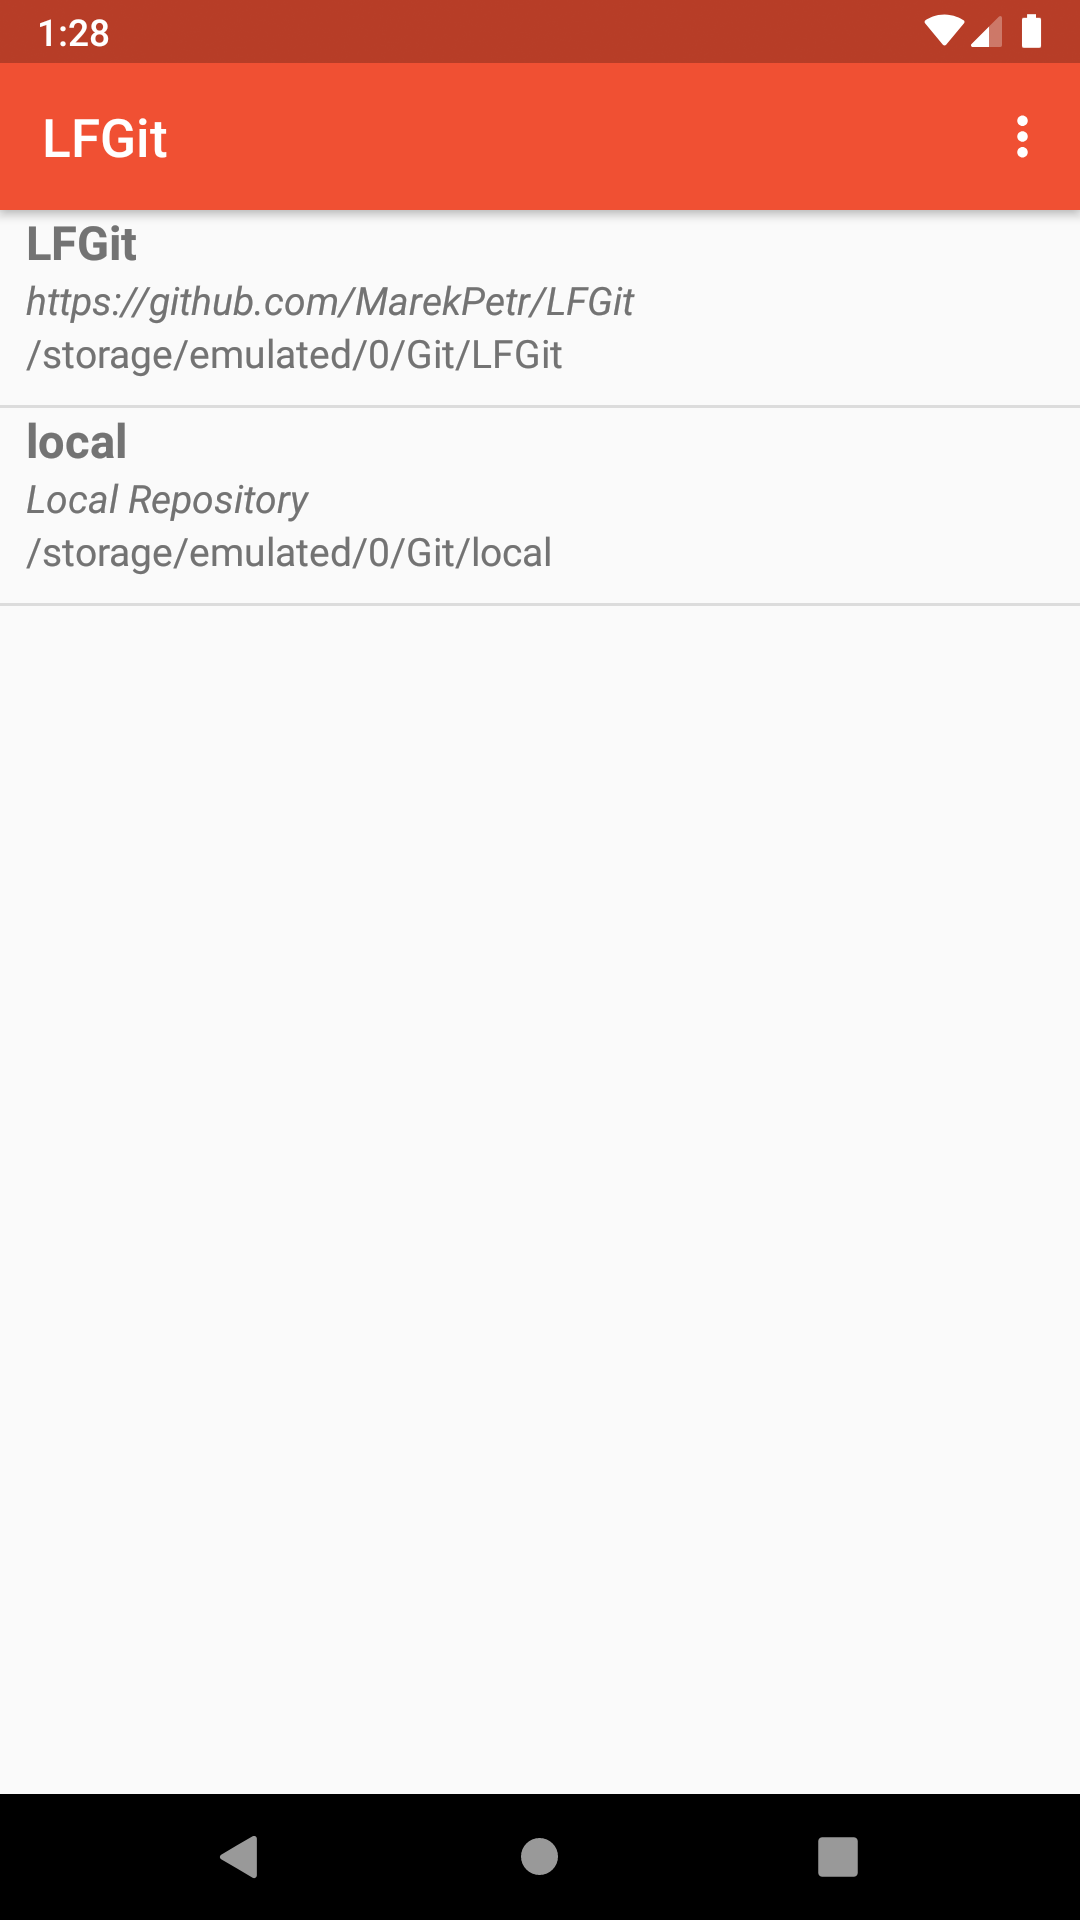
\includegraphics[width=5cm, keepaspectratio]{repo_list.png}}
        \caption{Seznam repozitářů}\label{fig:orig}
        \label{fig:repolist_frame}
    \end{subfigure}
    \begin{subfigure}{.4\textwidth}
        \centering
        \frame{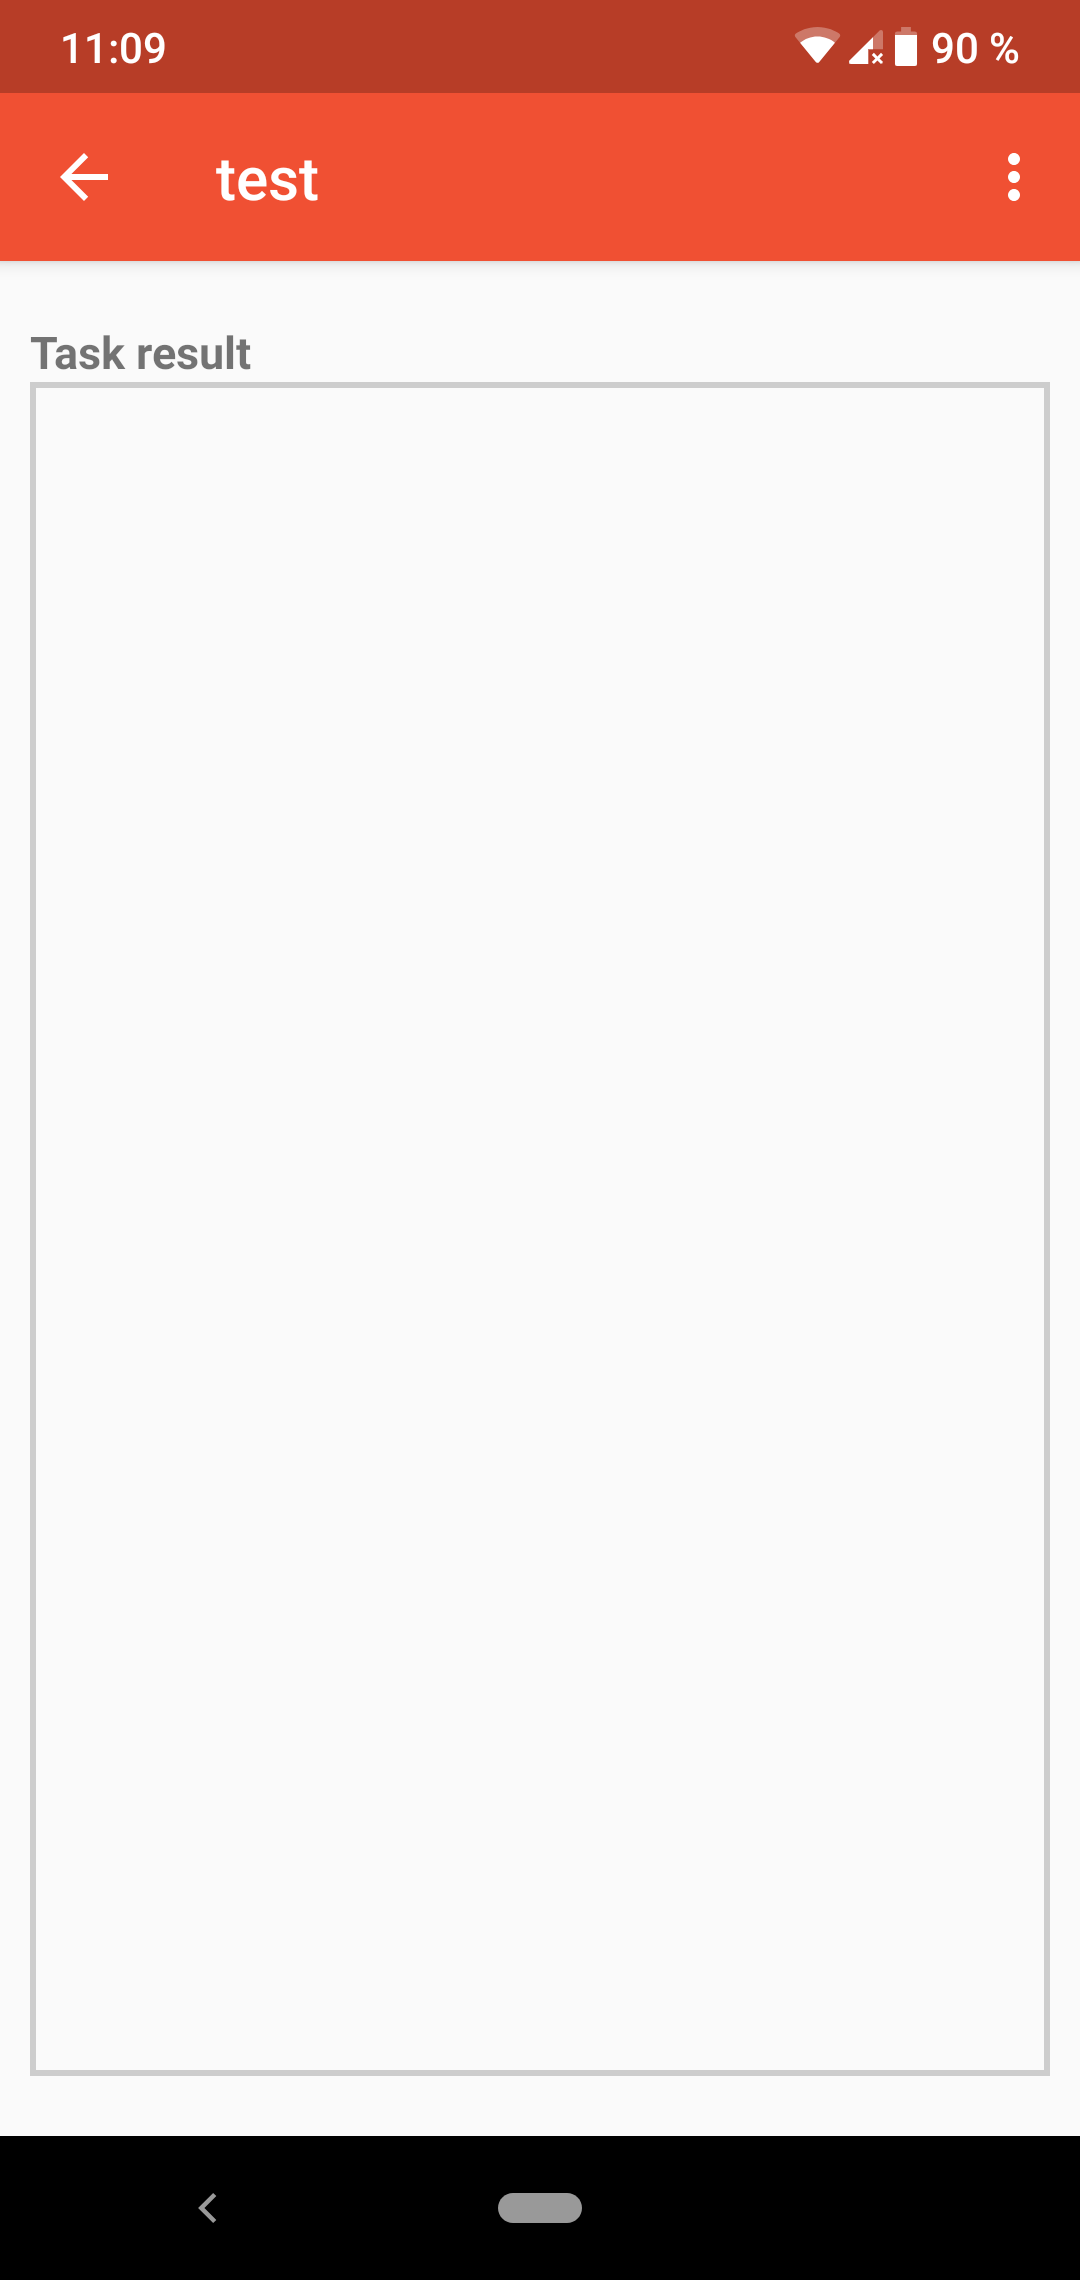
\includegraphics[width=5cm, keepaspectratio]{task_result.png}}
        \caption{Otevřený repozitář}
        \label{fig:result_frame}
    \end{subfigure}
\caption{Základní obrazovky}%
\label{fig:obrazovky}%
\end{figure}

Snímek~\ref{fig:repolist_frame} zobrazuje úvodní obrazovku aplikace. Nachází se na ní seznam repozitářů. U každého z nich jsou uvedeny jeho detaily. Jedná se o název repozitáře, jeho vzdálené umístění na serveru a místní cestu v zařízení. Pro přidání repozitářů a nastavení aplikace slouží menu v pravém horním rohu. 

Po otevření repozitáře aplikace přejde na druhou obrazovku~\ref{fig:result_frame}. Tam uživatel vykoná operace nad repozitářem. Ty budou dostupné v pravém draweru. Výsledky jednotlivých operací \emph{Gitu} budou vypisovány do \emph{Task result} pole.

\section{Manipulace se soubory}
Správce souborů je možné implementovat různými způsoby s různým stupněm jeho komplexnosti. Pro otevírání a editování souborů, včetně symbolických odkazů uživatel užije externí aplikace. Je mu tak ponechána volnost při volbě tohoto správce a předejde se hledání kompromisů pro jeho implementaci. Navíc aplikace  získá větší prostor pro ostatní funkce a uživatelské rozhraní se zjednoduší. Nevýhodou může být chybějící přehledný výběr souborů pro funkce, které pracují s jednotlivými soubory. Ale i s tím lze v aplikaci pracovat využitím \emph{SAF~\footnoteURL{https://developer.android.com/guide/topics/providers/document-provider}}.

\section{Možné způsoby integrace binárních souborů}
Jak již bylo zmíněno, aplikace pro příkazy \emph{Gitu} využívá binárních souborů. Ty je samozřejmě nejprve nutné do prostoru aplikace nějakým způsobem přenést. Z důvodu architektury systému Android není tato operace tak přímočará jako například na desktopovém systému Linux. Existují zde dvě možnosti. První je využití nativní knihovny o jejíž přenos a spouštění se postará systém Android. Druhá možnost je tyto operace provádět v rámci aplikace po instalaci balíčku.

    \subsection{Nativní knihovny}
    Z implementačního pohledu nejjednodušší způsob je první možnost. Tedy užití binární knihovny s příponou \emph{.so}. Tuto knihovnu je třeba v rámci struktury aplikace umístit do správného adresáře a systém Android si s její instalací poradí během samotné instalace aplikace. Tato metoda je dobře aplikovatelná v případě, že máte k dispozici staticky linkované binární soubory se strojovým výstupem. Z nich je pak snadné za použití Android NDK~\footnoteURL{https://developer.android.com/ndk} a JNI~\footnoteURL{https://developer.android.com/training/articles/perf-jni} vytvořit funkce, které lze používat přímo v kódu a získávat tak z těchto knihoven jejich výstup. Staticky linkované binární soubory v sobě obsahují všechny potřebné závislosti a jejich použití je tak možné samostatně. Lze jim tedy jednoduše přiřadit potřebnou příponu a budou zcela funkční. Získat tyto soubory je možné například křížovou kompilací daného programu. Staticky linkovaný \emph{Git} je možné zkompilovat využitím již existujících nástrojů~\footnoteURL{https://github.com/EXALAB/git-static}. Problém s tímto způsobem tkví v tom, že takto získaný binární soubor nelze jednoduše modifikovat. Je nutné ho pokaždé znovu zkompilovat, což je časově velice náročné. Navíc tyto binární soubory musí obsahovat veškeré knihovny, které pro svůj běh potřebují. Tedy při použití více těchto binárních souborů dochází k jejich redundanci.

    \newpage
    \subsection{Vlastní binární soubory}\label{subsec:dyn_binaries}
    Druhá možnost je využít binárních souborů dynamicky linkovaných a jejich spouštění implementovat v rámci aplikace. Tyto binární soubory nemají jejich závislosti obsažené přímo v nich samých, ale hledají je v daných umístěních. Tím dochází k úspoře místa. Také jsou jednoduše rozšiřitelné. Tento způsob řešení ale není pro zařízení Android zcela běžný a přináší tak další řadu problémů. Předně je nutné mít je zkompilované pro pevně danou cestu a správně nastavovat systémové proměnné. Dále tyto soubory nelze spouštět přes rozhraní JNI, ale dosáhne se toho využitím tříd, které vytváří vlastní proces na základě dodaných parametrů. Těmi jsou například metoda \code{exec} třídy \code{Runtime}~\footnoteURL{https://developer.android.com/reference/java/lang/Runtime} nebo právě již zmíněná metoda \code{command} třídy \code{ProcessBuilder}~\footnoteURL{https://developer.android.com/reference/java/lang/ProcessBuilder}. Toto spouštění i následné čtení výsledků je nutné provádět na samostatném vlákně a implementace tak není zcela triviální.

\section{Návrh integrace binárních souborů}
Pro tuto aplikaci bylo použito dynamicky linkovaných binárních souborů s vlastní instalací i spouštěním. Lépe se s nimi pracuje a aplikace tak bude lépe do budoucna rozšiřitelná. Navíc je velké množství dynamicky linkovaných programů již připraveno pro kompilaci prostřednictvím \emph{Termux-packages}~\footnoteURL{https://github.com/termux/termux-packages/}. Pro samotné spouštění bylo využito třídy \code{ProcessBuilder}. Je snadno použitelná a umožňuje intuitivní nastavování různých parametrů běhu procesu.

\section{Aplikační binární rozhraní - ABI}
 Různá zařízení Android mají osazeny různé procesory, které podporují různé sady instrukcí. Viz sekce \ref{sec:zaklady_abi}. Každá taková kombinace procesoru a instrukční sady má vlastní aplikační binární rozhraní - \emph{ABI}~\footnoteURL{https://developer.android.com/ndk/guides/abis}. Většina fyzických zařízení používá architekturu \emph{arm}~\footnoteURL{https://handstandsam.com/2016/01/28/determining-supported-processor-types-abis-for-an-android-device/}. Pro ladění aplikací se používá Android emulátorů a ty naopak pro nejlepší výkon používají architekturu \emph{x86}. Pro vydání aplikace na \emph{Google Play} je nutné, aby aplikace podporovala 32-bitové i 64-bitové verze dané architektury. Proto aplikace podporuje obě architektury pro obě verze. Jelikož by takto vytvořený \emph{APK} balíček byl příliš velký, aplikace používá pro distribuci formát \emph{Android App Bundle}~\footnoteURL{https://developer.android.com/guide/app-bundle}.
    
%-----------------------------------CHAPTER------------------------------------
\chapter{Implementace}
Po návrhu řešení aplikace následuje implementační část. V předchozí kapitole zabývajícím se návrhem byly popsány základní části aplikace, využité nástroje a architektura vývoje. Tato kapitola pojednává o postupu vývoje aplikace od získání binárních souborů po samotné vydání aplikace.

\section{Získání spustitelných binárních souborů}
Následující text rozebírá postup získání binárních souborů pro účely příkazů \emph{Gitu}, způsob jejich instalace a spouštění.

    \subsection{Kompilace binárních souborů}
    Jak již bylo zmíněno při návrhu, binární soubory jsou zkompilovány využitím repozitáře \emph{Termux-packages}~\footnoteURL{https://github.com/termux/termux-packages/}. Ten pro tento účel poskytuje obraz \emph{Dockeru}. Pro jeho použití pro jinou aplikaci je nutné upravit skript \code{scripts/build/termux\_step\_setup\_variables.sh} tak, aby cesta ke spustitelným souborům odpovídala cílové aplikaci. Při kompilaci pro tuto aplikaci byla nastavena cesta \code{TERMUX\_PREFIX} na \code{/data/data/com.lfgit/files/usr}. Takto byly zkompilovány binární soubory pro \emph{Git} i \emph{Git LFS}. \emph{Git Annex} touto cestou bohužel získat nelze. Jeho kompilace je velice problémová a přes veškeré úsilí se nakonec nepodařila. Další informace a provedený postup naleznete v sekci~\ref{sec:problemy_annex}.

    \subsection{Instalace binárních souborů}
    Pro instalaci binárních souborů bylo využito třídy \code{TermuxInstaller} aplikace Termux~\footnoteURL{https://github.com/termux/termux-app/blob/master/app/src/main/java/com/termux/app/TermuxInstaller.java}. Ta řeší podobný problém při instalaci linuxového prostředí a využití části metody \code{setupIfNeeded} vyřešilo problémy s instalací symbolických odkazů do aplikaci. Běžné kopírování souborů, jehož metody jsou popsány například zde~~\footnoteURL{https://www.baeldung.com/java-copy-file} totiž kopírují soubory, na které tyto symbolické soubory ukazují a tím dochází k jejich redundanci a nabývání velikosti instalace. Tato část byla implementována třídou \code{installTask} v balíčku \code{install}.

    Tento postup instalace vyžaduje užití \emph{Android NDK}~\footnoteURL{https://developer.android.com/ndk/} pro získání zdroje dat ze zkomprimovaného souboru ve formátu \emph{ZIP}. Ty jsou využity jak pro snížení velikosti, tak pro snadnou implementaci načtení a přenosu souborů.

    Po kompilaci byly smazány některé nepotřebné soubory zvětšující velikost instalace. Dále bylo třeba vygenerovat seznam symbolických odkazů pro všechny architektury. Ten byl vygenerován příkazem \code{find . -type l -ls > SYMLINKS.txt}. Poté byl tento seznam upraven tak, aby odpovídal formátu \code{$\hbox{symlink} \rightarrow \hbox{file}$}. Třída \code{installTask} byla upravena tak, aby s tímto formátem pracovala. Soubor \code{SYMLINKS.txt} byl dále připojen ke složce s binárními soubory dané architektury. Celá tato složka byla zkomprimována a archiv přesunut do složky \code{cpp}. Z těchto archivů se poté během instalace aplikace za pomocí \emph{Android NDK} kopírují soubory do zařízení.

    \subsection{Spouštění binárních souborů}
    Jak již bylo zmíněno~\ref{subsec:dyn_binaries}, aplikace používá pro spouštění spustitelných souborů \code{Process Builder}. Ten je implementován metodou \code{run} třídy \code{BinaryExecutor}. \code{Process Builder} se sice postará o vytvoření nového procesu, ale pokud po jeho ukončení očekáváme nějaký výstup, nemůže se samozřejmě běh aplikace během čekání blokovat. Proto se tyto příkazy spouští na samostatném vlákně a výsledek se předává prostřednictvím příslušného \emph{callbacku}, tedy zpětného volání. Toto zpětné volání je implementováno rozhraním \code{ExecListener} třídy \code{executors}. Toto rozhraní poté implementuje třída, která očekává výsledek daného volání.

\section{Aplikace}
Po implementaci spouštění binárních souborů přichází na řadu implementace samotné aplikace. Základní popis implementace stěžejních částí je rozdělen podle jednotlivých obrazovek aplikace.

    \subsection{Seznam repozitářů}
    Uvítací obrazovka je implementována aktivitou \code{RepoListActivity}. Ta při prvním spuštění nainstaluje potřebné binární soubory a dále zobrazí prázdný seznam repozitářů. Tento seznam zobrazuje aktuální stav databáze repozitářů. Repozitář uživatel do seznamu přidá prostřednictvím menu. Vybraná akce spustí daný \emph{Intent} a přesune uživatele na další obrazovku. Mezi tyto akce patří i přidání  repozitáře. Přidané repozitáře jsou také synchronizovány s úložištěm. V případě smazání z úložiště dojde při dalším načtení tohoto seznamu k jeho smazání ze seznamu a tedy i databáze. Obnovení seznamu lze provést i okamžitě gestem táhnutí shora dolů. V případě smazání repozitáře v době jeho otevření, bude uživatel na toto upozorněn při provádění příkazů \emph{Gitu} a navrácen zpět do seznamu repozitářů. 

    \subsection{Přidání repozitáře}
    Repozitář lze do seznamu přidat třemi způsoby. Pokud již existuje v paměti zařízení, lze ho přidat tlačítkem menu \code{Add repository}. Tato akce spustí \emph{intent} pro vybrání složky s repozitářem. Dále je možné repozitář inicializovat a klonovat. Obrazovka s klonování a inicializací je implementována aktivitou \emph{AddRepoActivity}. Také je podporováno mělké klonování pro zadaný počet \emph{commitů}, tedy hloubku. 

    \subsection{Provedení příkazů \emph{Gitu}}
    Po kliknutí na repozitář dojde k jeho otevření. V pravém bočním panelu se nachází seznam všech podporovaných příkazů. Ten je implementován třídou \code{RepoTasksAdapter}. Při kliknutí na příkaz dojde k zavolání metody \code{execGitTask} do \code{RepoTasksViewModelu}. Ta z pole příkazů implementovaného rozhraním \code{GitAction} vybere podle polohy v panelu správný příkaz a vykoná ho.

\section{Problémy objevené při implementaci}\label{sec:problemy_implem}
Implementace provázelo velké množství překážek. Ty se začaly objevovat již při procesu získání binárních souborů a jejich řešení nebylo vždy snadné. Následující text se bude věnovat nejzajímavějším problémům, které nejsou při vývoji zcela běžné.

    \subsection{Příkazy Gitu}
    Logika příkazů \emph{Gitu} je implementována ve \emph{view modelech} daných aktivit. Jelikož všechny volané funkce vrací hodnotu zpětným voláním, bylo nutné pro získání všech vstupů pro vykonání daného příkazu definovat stavy jeho zpracování. K tomu slouží třída \code{TaskState}. Obsahuje atribut \code{mInnerState} určující aktuální stav rozpracovaného příkazu a atribut \code{mPendingTask} definující zpracovávaný příkaz. Existují zde dva speciální stavy atributu \code{mInnerState} \code{FOR\_APP} a \code{FOR\_USER}. Jsou to stavy, které určují, jestli bude výsledek následujícího příkazu zobrazen uživateli, či bude využit jako vstupní argument pro jiný účel aplikace.

        \subsubsection{Push}
        Nejsložitější příkaz na implementaci je příkaz \emph{push}. Ten pro přístup do vzdáleného repozitáře potřebuje jak jeho \emph{URL}, tak přihlašovací údaje uživatele. Ty jsou žádány pro každý nově přidaný repozitář pouze při prvním vykonávání tohoto příkazu. Po jejich zadání jsou uloženy v databázi v tabulce daného repozitáře. Databáze je uložena ve vnitřním prostoru aplikace, kam má přístup jen ona samotná. Uložení těchto citlivých údajů je tedy relativně bezpečné. Před provedením příkazu jsou znaky uživatelského jména a hesla kódovány do \code{application/x-www-form-urlencoded} MIME formátu~~\footnoteURL{https://developer.android.com/reference/java/net/URLEncoder}.\\ Samotné provedení pak probíhá prostřednictvím \emph{http} nebo \emph{https} protokolu a to příkazem \code{git push http(s)://username:password@domain}.
        Tento způsob aplikace používá z důvodu nemožnosti zadávat vstupní data binárním souborům během jejich běhu. \emph{ProcessBuilder} sice umožňuje před spuštěním programu zadat vstupní data, ale není možné v rámci běhu reagovat na čtení vstupů z příkazové řádky tak jako při využití terminálového rozhraní.

        \newpage
        \begin{figure}[h]
            \centering
            \vspace{0.5cm}
            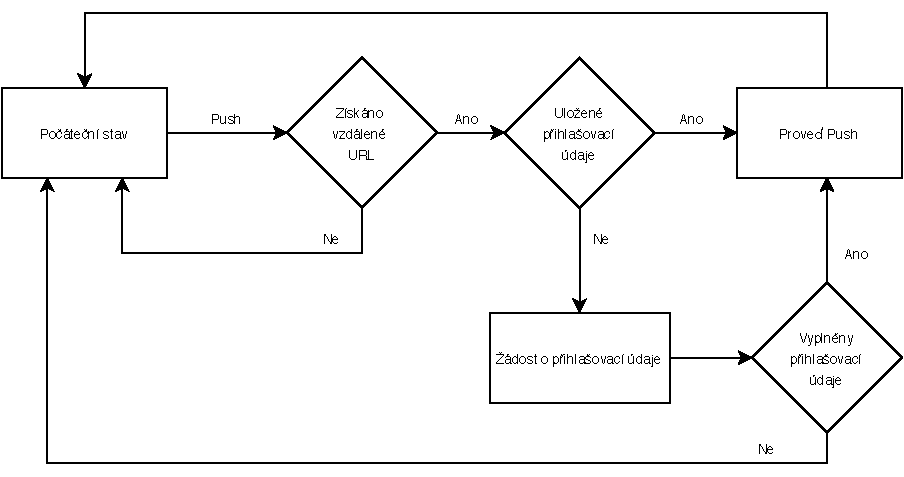
\includegraphics[]{drawio/push_diagram.pdf}
            \caption[Diagram provedení příkazu push]{Zjednodušený diagram provedení příkazu push.}
            \label{diagram:push}
        \end{figure}
    
    \subsection{Správce souborů}
    Implementace užití externího správce souborů se ukázala jako více problematická, než se při návrhu předpokládalo. Původní návrh této funkcionality spočíval v předání \emph{URI} externí aplikaci správce souborů, kterou uživatel používá jako výchozí. Toho nebylo možné dosáhnout z důvodu použití rozdílných typů \emph{URI} existujících aplikací správce souborů. Pro jeho zahrnutí do aplikace by tak bylo nutné implementovat vlastní správce. Toho se aplikace snažila z mnoha důvodů již od návrhu vyhnout. Zejména proto, že různí uživatelé budou mít na tento správce různé požadavky. Proto byl prostor aplikace plně věnován prostředí \emph{Git}. Uživatel tak obdobně jako při užití na desktopových systémech bude přecházet z jedné aplikace do druhé. To pro pokročilého uživatele systému \emph{Android} a \emph{Git}, na kterého tato aplikace cílí, nepředstavuje překážku.
    Toto rozhodnutí je podpořeno také faktem, že samotné užití programu \emph{Git} neřeší žádný komplexní problém uživatele. Ten proto bude používat řadu dalších aplikací, které v kooperaci splní jeho cíl.

    \newpage
    \subsection{Git LFS}\label{sec:problemy_lfs}
    S implementací tohoto rozšíření \emph{Gitu} se pojily dva problémy. První se týká samotné integrace do prostředí systému \emph{Android}, druhý pak mechanismu \emph{Git Hooks}\footnoteURL{https://git-scm.com/book/en/v2/Customizing-Git-Git-Hooks}.

    \emph{Hooks}, neboli háček, \emph{Gitu} umožňuje před nebo po vykonání jeho příkazu spustit z definovaného adresáře daný skript. \emph{Git LFS} tohoto mechanismu využívá pro synchronizaci repozitáře.

    \subsubsection{Integrace do aplikace}
    Integraci tohoto rozšíření provázely problémy, ale všechny byly řešitelné. Neobvyklý problém nastal při prvních pokusech o přidání sledovaného souboru do \emph{stage}. \emph{Git LFS} při něm zobrazoval chybou hlášku, že není možné vytvořit podproces pro spuštění jeho programu \code{filter-process}. Pro zjištění možné příčiny byl příkaz \code{git add .} spuštěn prostřednictvím ladícího programu \emph{strace}~\footnoteURL{https://strace.io/}. Pro jeho užití bylo nutné výstup přesměrovávat do souboru. \code{StringBuilder}, který je v aplikace využit pro zpracování výstupu z binárních programů již tak rozsáhlý výstup nezvládal zpracovávat a vracel jen jeho část. Ani samotný \emph{strace} ale nebyl nic platný. Na žádnou chybu neupozornil.
    
    Pro řešení bylo přidána tzv. \emph{issue} v oficiálním repozitáři \emph{Git LFS}~\footnoteURL{https://github.com/git-lfs/git-lfs}. S pomocí jednoho z hlavních vývojářů tohoto programu byl problém vyřešen. Využitím přepínače \code{strace '-f'} bylo zjištěno, že \emph{Git LFS} nenalezl \emph{shell}. Problém byl vyřešen mírnou oklikou a to přidáním symbolického odkazu na \code{/system/shell} do složky \code{bin}, kde byl tento interpret očekáván.

    \subsubsection{Git LFS hooks}~\label{subsub:problemy_git_hooks}
    Integrací problémy s Git LFS stále nekončily. Při vykonávání kteréhokoliv příkazu, který spouštěl tzv. \emph{hook}, \emph{Git} vracel chybu pro nedostatečná práva pro otevření těchto souborů.
    
    Bylo to dáno tím, že příkaz pro instalaci \emph{Git LFS} do repozitáře, vytvářel \emph{hooky} uvnitř tohoto repozitáře, ale nepřiřadil jim patřičná práva. Řešení byla možná dvě. Buď po proběhnutí každé instalace nastavit práva těmto souborům ručně, nebo tyto hooky vytvářet ve vnitřním prostoru aplikace, kde jsou již potřebná práva nastavena.
    
    Na první pohled by se mohlo zdát, že uživatelsky přívětivější je první řešení. Uživatel \emph{hooky} vytvoří jednou při instalaci \emph{Git LFS} a při klonování repozitáře na jiném zařízení již budou nainstalovány. Bohužel situace taková není. \emph{Hooky} jsou při výchozím nastavení umístěny lokálně ve složce \code{.git} repozitáře a při klonování zkopírovány nejsou~~\footnoteURL{https://www.atlassian.com/git/tutorials/git-hooks}.

    Z tohoto důvodu byla vybrána druhá varianta. \emph{Hooky} se vytváří automaticky ve vnitřním prostoru aplikace při její instalaci. Uživatel je tak nemusí instalovat manuálně v každém repozitáři zvlášť a to zjednoduší jeho práci.

    \newpage
    \subsection{Git annex}\label{sec:problemy_annex}
    Získávání spustitelných souborů pro \emph{Git Annex} se ukázalo jako velice problematické. Následující text je shrnutím mnoha provedených pokusů, z nichž některé byly velice blízko k získání těchto souborů, ale nakonec se to bohužel nepodařilo.

    \subsubsection{Oficiální distribuce pro Termux}
    Nejprve byly staženy instalační soubory \emph{Git Annex} z oficiální webové wiki stránky~~\footnoteURL{https://git-annex.branchable.com/Android/}. Tyto soubory byly nainstalovány do vnitřního prostoru aplikace s příslušnými právy pro spuštění. Při prvních pokusech byly zjištěny problémy týkající se chybějících programů interpretu shellu. Pro jejich vyřešení byl stažen program \emph{Busybox}~\footnoteURL{https://busybox.net/} pro architekturu testovacího zařízení. Ten problém nevyřešil, jelikož z nějakého důvodu nebylo možné ho spustit. Proto byly potřebné skripty přepsány do podoby, kterou shell zařízení byl schopný zpracovat. Později se zjistilo, že používaná verze \emph{Busyboxu} byla vadná a problém vyřešila jiná verze, ale tento program už nebyl potřeba. Přes přepsání všech inkriminovaných příkazů skriptů \emph{Git Annexu} se nedařilo tento program spustit. Užitím programu \emph{strace} bylo zjištěno, že bezpečnostní zabezpečení Android tzv. \emph{Seccomp} filtrování zamezuje spuštění určitého kódu spojeného s jeho spuštěním. Na tento problém již narazil i Joe Hess, vývojář \emph{Git Annexu} při jeho portování na \emph{Termux} Androidu. Po prozkoumání jeho řešení bylo zjištěno, že řešení leží v nástroji zvané \emph{Proot}, která toto filtrování umí obejít. Bohužel ani po mnoha pokusech spouštění \emph{Git Annexu} tímto nástrojem nebylo dosaženo kýženého výsledku.

    \subsubsection{Vlastní kompilace Git Annex}
    Dále následovalo mnoho pokusů o vlastní křížovou kompilaci \emph{Git annexu}. Jeho kód je psán v jazyce \emph{Haskell} a tato kompilace je tím značně zkomplikována. Byly provedeny pokusy o kompilace pomocí nástroje \emph{Nix}~\footnoteURL{https://github.com/pololu/nixcrpkgs}, \emph{GHC Android}~\footnoteURL{https://medium.com/@zw3rk/a-haskell-cross-compiler-for-android-8e297cb74e8a} a dalších. Některé pokusy selhaly již při kompilaci křížového kompilátoru, jiné až při kompilaci \emph{Git Annexu}.

    \subsubsection{Vlastní kompilace nástroje Proot}
    Jelikož nebylo skrze křížovou kompilaci dosaženo většího pokroku než užitím verze určené pro \emph{Termux}, další pokusy pokračovaly právě s ní. Na pomoc s problémem s \emph{Proot} byla kontaktována jeho komunita na jeho komunikačním kanále služby \emph{Gitter}~\footnoteURL{https://gitter.im}. S pomocí těchto vývojářů se podařilo zkompilovat verzi \emph{Prootu}, kterou používá \emph{Termux} pro prostředí balíčku vyvíjené aplikace. To vyřešilo problém s \emph{Seccomp} filtrováním, ale objevil se další. \emph{Git annex} stále nebylo možné spustit. Problém se týkal chybějících programů interpretu. \emph{Termux} pro běh programů vytváří vlastní linuxový systém, kde jsou nainstalovány všechny standardní programy. Toto prostředí mu tato aplikace neposkytuje. Tento fakt byl pro funkci skriptů obejit jejich přepsáním. Pro binární soubory toto bohužel možné není. Implementace vlastního systém uvnitř aplikace je velice problémová a také náročná na úložiště. Tento problém nakonec nebyl vyřešen. Všechny zdroje byly investovány do vývoje kvalitní aplikace bez podpory \emph{Git Annexu} s možností rozšíření po jejím vydání, v případě nalezení řešení.

%-----------------------------------CHAPTER------------------------------------
\chapter{Testování}
Testování aplikace probíhalo manuálně a to ve dvou fázích.
\section{Příkazy Gitu}
První fáze testování byla zaměřena na správné provedení příkazů \emph{Gitu}. Při tomto testování byly nad repozitáři spouštěny různé příkazy a jejich výsledek byl konfrontován se stavem repozitáře. Aktuální stav repozitáře se ověřoval využitím aplikace \emph{Termux}, zpětnou kontrolou na serveru \emph{GitHub} i klonováním repozitáře do jiných zařízení při použití této aplikace. Tím bylo dosaženo zajištění funkčnosti těchto příkazů.

Testována byla také schopnost provedení základního vytvoření repozitáře a jeho \code{push} na nově vzniklý prázdný vzdálený repozitář. Při tomto kroku byl opravován zejména samotný příkaz \code{push}. Ten byl testován na různé formy \emph{URL}, uživatelského jména i hesla. Přidána byla kontrola na zadání \emph{http(s)} adresy, jelikož i autentizace probíhala touto cestou. Uživatelská jména a hesla byla pro ověření správného \emph{URL} kódování testována na speciální znaky.

Opravy se dotkly i rozšíření \emph{Git LFS}. Během testování bylo využito například příkazů \emph{git-lfs env} nebo \emph{git-lfs status}. Tyto příkazy byly poté pro jejich užitečnost přidány do příkazů aplikace.

\emph{Git LFS} také zpočátku neposílalo obsah sledovaných souborů na server, ale pouze jejich odkaz. Ten byl při stažení na jiná zařízení neplatný. Tento problém se týkal \emph{Git LFS hooks} a byl již popsán v sekci~\ref{subsub:problemy_git_hooks}.

\section{Uživatelské rozhraní}
Otestováno bylo i uživatelské rozhraní. Testováno bylo přerušení započatých sekvencí, které předchází různým příkazům tak, aby se tyto prvky chovaly validně. To mimo jiné zahrnovalo testy správného stavu zobrazení různých formulářů i po změně rozložení displeje nebo jejich skrytí na pokyn aplikace.

Upravovány byly i velikosti písma a některých jiných grafických prvků. Změnami také prošla obrazovka inicializace a klonování repozitáře. Ta při vodorovném režimu skrývala tlačítko pro spuštění klonování. Proto byla do aplikace přidána speciální verze pro vodorovné rozložení, které toto tlačítko posune do viditelné zóny obrazovky.
%-----------------------------------CHAPTER------------------------------------
\chapter{Závěr}